\documentclass[11pt]{amsart}


\usepackage[ibidtracker=false,uniquename=false,giveninits=true,terseinits=true,backend=biber]{biblatex}
\usepackage{float}
\usepackage{graphicx}
\usepackage{todonotes}
\usepackage{subcaption}
\usepackage{amsmath}
\usepackage{amsthm}
\usepackage{amssymb}
\usepackage{algorithm}
\usepackage[noend]{algorithmic}
\usepackage[foot]{amsaddr}
\usepackage[misc]{ifsym}
\usepackage{enumitem}
\usepackage{geometry}
\usepackage[hidelinks]{hyperref}

\renewbibmacro{in:}{}
\addbibresource{rnni_geometry.bib}
\AtEveryBibitem{
	\clearlist{language}
}

\setlist{leftmargin = 0pt}
\geometry{margin=1in}

\newtheorem{proposition}{Proposition}
\newtheorem{theorem}{Theorem}
\newtheorem{lemma}{Lemma}
\newtheorem{corollary}{Corollary}
\newtheorem{problem}{Problem}
\newtheorem{conjecture}{Conjecture}

\newcommand{\rnni}{\mathrm{RNNI}}
\newcommand{\findpath}{\textsc{FindPath}}
\newcommand{\mrca}{\mathrm{mrca}}
\newcommand{\rank}{\mathrm{rank}}
\newcommand{\nni}{\mathrm{NNI}}
\newcommand{\spr}{\mathrm{SPR}}
\newcommand{\tbr}{\mathrm{TBR}}
\newcommand{\fp}{\mathrm{FP}}
\newcommand{\np}{\mathbf{NP}}
\newcommand{\decprob}[1]{\rnni(#1)\text{-}\mathrm{SP}}
\newcommand{\rad}{\mathit{rad}}
\renewcommand{\O}{\mathcal O}
\renewcommand{\epsilon}{\varepsilon}
\renewcommand{\thesubfigure}{\Alph{subfigure}}

\newcommand{\summary}[1]{\textbf{#1}} % Print summaries to .pdf
% \newcommand{\summary}[1]{} % Hide summaries in .pdf

\graphicspath{{figures/}}

\sloppy


\title[Geometry of ranked tree spaces]{The Geometry of the Ranked Nearest Neighbour Interchange Space}
\date{\today}
\author{Lena Collienne}
\email{lcollienne@cs.otago.ac.nz}
\address{Department of Computer Science, University of Otago, New Zealand}
\author{Alex Gavryushkin\textsuperscript{\Letter}}
\email{\textsuperscript{\Letter}alex@biods.org}
\thanks{}

\begin{document}

\begin{abstract}
\end{abstract}

\maketitle


\section{Introduction}

\summary{Motivation -- ranked trees and tree rearrangements.}

\summary{More motivation, sepcifically for $\rnni$ and $\rho$.}

\summary{Why we want to investigate geometrical properties of $\rnni(\rho)$ for different $\rho$ and that we want to compare properties in spaces for different $\rho$.}

\summary{Structure of the paper.}


\section{Technical Introduction}

\summary{Defining the basics of ranked trees.}

Things we need to define:
\begin{itemize}
	\item with $\rnni$ we mean $\rnni(1)$ -- do we want to use this everywhere?
	\item $d(T,R)$ is the weight of a shortest path
	\item $\rnni(\infty)$
	\item rank interval for Lemma~\ref{lemma:nni_path_to_caterpillar}
	\item cherry (for lemma~\ref{lemma:max_dist_ctree})
\end{itemize}

\summary{Introduce $\findpath$ and that it computes $\rnni$ distances.}


\section{Caterpillar Trees}

\summary{The set of caterpillar trees is convex in $\rnni$.}
\begin{theorem}
	The set of caterpillar trees is convex in $\rnni$.
\end{theorem}

\summary{The set of caterpillar trees is convex in $\rnni(\rho)$ for $\rho > 1$.}
\begin{corollary}
	The set of caterpillar trees is convex in $\rnni(\rho)$ if and ony if $\rho \geq 1$.
\end{corollary}

\begin{proof}
	\begin{figure}[ht]
		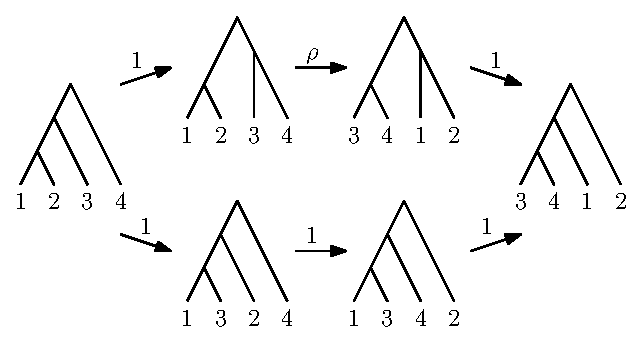
\includegraphics[width=0.5\textwidth]{caterpillar_non_convex.eps}
		\caption{A shortest caterpillar path between caterpillar trees $T$ and $R$ at the bottom and a path consisting of non-caterpillar trees at the top.
		The path at the top is shorter than the one at the bottom for all $\rho<1$.}
		\label{fig:caterpillar_non_convex}
	\end{figure}
\end{proof}


\section{Diameter and Radius}

\summary{Definition of Diameter and that we consider it depending on $\rho$.}
In this section we want to investigate the diameter of $\rnni(\rho)$, which is the greatest distance between any pair of vertices (trees) in this graph, i.e. $\max\limits_{\text{trees }T,R}d(T,R)$.
We will show that the diameter of $\rnni(\rho)$ depends on $\rho$.
Since the $\rnni$ graph, where rank moves have weight one, is the only one for which a polynomial time algorithm for computing distances is known, we start considering the diameter of this graph before turning to $\rnni(\rho)$ for different values of $\rho$.

\summary{Diameter in $\rnni$ follows from results in previous paper.}
The algorithm $\findpath$ of \autocite{collienne2020computing}, which computes distances in $\rnni$, facilitates finding the diameter of the $\rnni$ graph. 
\begin{corollary}
	The diameter of $\rnni$ is $\frac{(n-1)(n-2)}{2}$.
	\label{cor:diameter_rnni}
\end{corollary}

\begin{proof}
	The proof of Corollary 1 in \autocite{collienne2020computing} gives an example of trees for which the length of the path computed by $\findpath$, and therefore the distance, is $\frac{(n-1)(n-2)}{2}$.
	It remains to show that $\findpath$ cannot computes paths longer than $\frac{(n-1)(n-2)}{2}$.
	\todo{Explain that this cannot happen by explicitely mention how often while and for loop are executed -- do we want to repeat the pseudo-code in this paper?}
\end{proof}

Not only for $\rnni$, but also for $\rnni(0)$, we know the diameter from previous results.
As rank moves in $\rnni(0)$ weigh zero, the distance between two trees in this space is the same as the $\nni$ distance between these trees when ignoring ranks.
Therefore, these graphs have the same diameter.

\begin{proposition}
	The diameter of $\rnni(0)$ is $\Theta(n \log(n))$.
	\label{prop:diameter_nni}
\end{proposition}

\begin{proof}
	This follows from the diameter of the $\nni$ graph, which is known \autocite{Semple2003-nj} to be $\Theta(n \log(n))$.
\end{proof}

\summary{Results for $\rnni$ and $\rnni(0)$ give us bounds for the diameters of all spaces with $0 < \rho < 1$.}
With the previous results in Corollary~\ref{cor:diameter_rnni} and Proposition~\ref{prop:diameter_nni} we can infer bounds for diameters of spaces $\rnni(\rho)$ with $0 < \rho < 1$.
A path in $\rnni(\rho)$ between two trees corresponds to paths in $\rnni(0)$ and $\rnni(1)$ that contain the same moves, but have different total length, due to the different weighing of rank moves.
Therefore, the length of such a path is bounded from below by the length of the corresponding path in $\rnni(0)$ and from above by the corresponding path in $\rnni(1)$.
With Corollary~\ref{cor:diameter_rnni} and Proposition~\ref{prop:diameter_nni} it follows that the diameter of $\rnni(\rho)$ with $\rho < 1$ is bounded from below by $\Theta(n \log(n))$ and from above by $\frac{(n-1)(n-2)}{2}$.

\summary{Diameter of $\rnni(\rho)$ for $\rho > 1$.}
So far $\rnni(\rho)$ for $0 \leq \rho \leq 1$ has been the centre of our investigation of diameters.
We now continue by considering spaces $\rnni(\rho)$ for $\rho > 1$, where rank moves are more expensive than $\nni$ moves.
Specifically, we give an upper bound for the diameter of $\rnni(\infty)$ from which we can follow that all spaces $\rnni(\rho)$ have a diameter less or equal to this bound.
Before this, however, we need to observe that for $\rnni(\infty)$ every pair of trees is connected by a path consisting of $\nni$ moves only.

\begin{lemma}
	In $\rnni$ every tree is connected to a caterpillar tree by a path that consists of $\nni$ moves only.
	\label{lemma:nni_path_to_caterpillar}
\end{lemma}

\begin{proof}
	We prove this lemma for a given tree $T$ by induction on the number $i$ of rank intervals of $T$.
	In the base case $k = 0$ the tree $T$ is a caterpillar tree and the statement is true.
	For the induction step we assume that $T$ has $i+1$ rank intervals and all trees with less than $i+1$ rank intervals are connected to a caterpillar trees through a sequence of $\nni$ moves.
	We now construct a series of $\nni$ moves that, starting at $T$, ends in a tree that has less than $i+1$ rank intervals.
	Let the node of rank $k+1$ in $T$ be the highest ranked node incident to a rank interval.
	This means that the interval given by nodes of rank $k$ and $k+1$ is a rank interval and all intervals above $(T)_{k+1}$ are edges.
	Let $(T)_l$ be the parent of $(T)_k$.
	Hence $l > k+1$, and $[(T)_{l-1}, (T)_{l}]$ is an edge.
	On this edge an $\nni$ move can be performed that results in a tree $T'$ in which the rank of the parent of $(T')_k$ is $l-1$, as depicted in Figure~\ref{fig:nni_path_caterpillar}.
	In the tree $R$ resulting from iteratively repeating this until $l = k+1$ the parent $(R)_k$ has rank $k+1$.
	Hence the rank interval bounded by nodes of rank $k$ and $k+1$ in $T$ turned into an edge while all intervals above $k+1$ remain edges in $R$.
	As $R$ has one rank interval less than the $i+1$ rank intervals of $T$, the induction hypothesis can be applied to $R$.
	This gives a sequence from $T$ to a caterpillar via $R$ that consists of $\nni$ moves only.
	\begin{figure}[ht]
		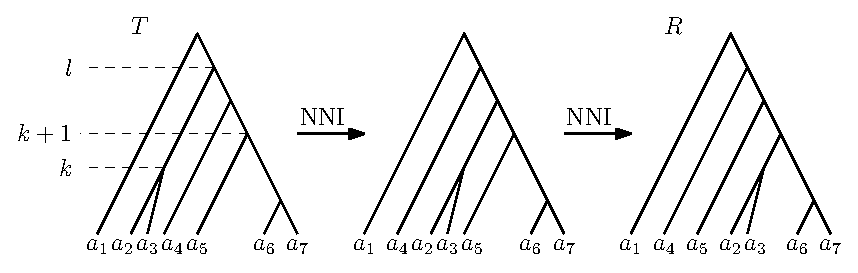
\includegraphics[width=0.8\textwidth]{nni_path_caterpillar.eps}
		\caption{Example of a tree $T$ with two rank intervals and a sequence of $\nni$ moves that results in a tree $R$ with one rank interval as described in the proof of Lemma~\ref{lemma:nni_path_to_caterpillar}.}
		\label{fig:nni_path_caterpillar}
	\end{figure}
\end{proof}

With this lemma we are able to prove that the diameter of $\rnni(\infty)$ is quadratic in $n$.
\begin{corollary}
	The diameter of $\rnni(\infty)$ is less or equal to $3 \frac{(n-1)(n-2)}{2}$.
\end{corollary}

\begin{proof}
	Let $T$ and $R$ be two trees in $\rnni(\infty)$.
	With Lemma~\ref{lemma:nni_path_to_caterpillar} we know that any tree can be connected to a caterpillar tree by a sequence of $\nni$ moves.
	Moreover, the proof of the lemma implicitly proposes an algorithm to convert a tree into a caterpillar tree by removing rank intervals by a top-down approach.
	We show that the paths from a tree to a caterpillar tree that are given by this algorithm have at most length $\frac{(n-1)(n-1)}{2}$.
	Since we also know that the set of caterpillar trees is convex in $\rnni$ \todo{reference -- maybe we should have the caterpillar section before this one?}, and hence the maximum distance between caterpillar trees is bounded by the diameter $\frac{(n-1)(n-2)}{2}$ of $\rnni$ (Corollary~\ref{cor:diameter_rnni}), this corollary follows.

	For finding the maximum length of a path computed by the algorithm suggested in the proof of Lemma~\ref{lemma:nni_path_to_caterpillar}, we consider every iteration (induction step).
	In each of these, at least one rank interval turns into an edge.
	The number of $\nni$ moves needed for this depends on the rank of the upper node bounding the rank interval.
	If we assume the worst case, that is, every interval except for the edge $[(T)_{n-1},(T)_{n-2}]$ is a rank interval, then there are $i$ $\nni$ moves needed in iteration $i$.
	Since there are $n-2$ iterations, it follows that at most $\frac{(n-1)(n-2)}{2}$ $\nni$ moves are needed to get from an arbitrary tree to a caterpillar tree.
	\todo{I suspect writing the algorithm down properly and using it to prove Lemma~\ref{lemma:nni_path_to_caterpillar} and this corollary might be easier than this. This explanation of the 'implicitly' defined algorithm is not sufficient.}
\end{proof}

\summary{Radius of $\rnni$ is equal to its diameter.}
For proving that the radius of $\rnni$, which is defined $\min\limits_{\text{tree } T}\max\limits_{\text{tree }R} d(T,R)$, equals its diameter, we need the following lemma.
\todo{Can we come up with a more intuitive description of what the radius of a graph is?}

\begin{lemma}
	For every tree on $n$ leaves exists a caterpillar tree with distance $\frac{(n-1)(n-2)}{2}$ from it in $\rnni$.
	\label{lemma:max_dist_ctree}
\end{lemma}

\begin{proof}
	We prove this lemma by induction on the number of leaves $n$.
	The base case $n=3$ is trivial, as all three trees in this space are caterpillar trees with distance one.
	For the induction step we consider an arbitrary tree $T$ with $n + 1$ leaves.
	Let $T'$ be the tree on $n$ leaves resulting from deleting one of the cherry leaves, which we denote by $x$, of $T$.
	By applying the induction hypothesis on $T'$ we can find a caterpillar tree $R'$ that has distance $\frac{(n-1)(n-2)}{2}$ to $T'$.
	Now consider the tree $R$ resulting from adding the leaf $x$ at the top of $R'$ such that the root of $R$ has $x$ and $R'$ as children.

	In the first iteration of $\findpath$ the leaf $x$ moves down by $\nni$ moves until it reaches the second cherry leaf $y$ of $T$ and builds a cherry with it, which then is moved down by rank swaps as depicted in Figure~\ref{fig:max_dist_ctree}.
	There are $n-1$ $\rnni$ moves needed for this as $(x,y)_R$ moves down from the root with rank $n$ to the cherry of rank one.
	The tree at the end of this first iteration on $\fp(T,R)$ is equals $R'$ when ignoring the leaf $x$ and its parent.
	Since the cluster $\{x,y\}$ is not considered again in $\findpath$, the remaining part of $\fp(T,R)$ contains the same moves as $\fp(T',R')$ from which we can follow that $|\fp(T,R)| = |\fp(T',R')| + n-1$.
	\todo{Is it OK to phrase it like this?}
	Therefore it is $d(T,R) = \frac{(n-1)(n-2)}{2} + n-1 = \frac{n(n-1)}{2}$, which proves the lemma.
	\begin{figure}[ht]
		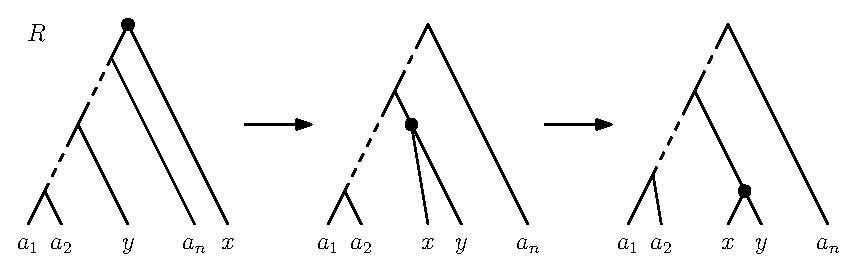
\includegraphics[width=0.8\textwidth]{max_dist_ctree.eps}
		\caption{Initial $n - 1$ $\rnni$ moves of $\fp(R,T)$ as described in the proof of Lemma~\ref{lemma:max_dist_ctree}.
		Removing the leaf $x$ and suppressing the non-root node of degree two from the tree on the right results in $R'$ as described in the lemma.}
		\label{fig:max_dist_ctree}
	\end{figure}
\end{proof}

\begin{proposition}
	The radius of the $\rnni$ graph equals its diameter, i.e. $\rad(\rnni) = \frac{(n-1)(n-2)}{2}$.
\end{proposition}

\begin{proof}
	From Lemma~\ref{lemma:max_dist_ctree} we know that there is a tree with distance $\frac{(n-1)(n-2)}{2}$ from any given tree.
	Hence the radius equals the diameter of $\rnni$.
\end{proof}

\summary{Radius of $\rnni(\rho)$ for other values of $\rho$.}


\section{Cluster Property}

\summary{Why the Cluster Property is relevant.}

\summary{$\rnni$ has the cluster property.}
\begin{theorem}
	The $\rnni$ graph has the cluster property.
\end{theorem}

\summary{$\rnni(0)$ does not have cluster property.}
\begin{proposition}
	$\rnni(0)$ does not have the cluster property.
\end{proposition}

\summary{Cluster Property of $\rnni(\rho)$ for $\rho \neq 0, 1$?}


\section{Generalisation}

\summary{All (?) results from $\rnni$ transfer to discrete time-trees.}

\summary{How partition lattices correspond to $\rnni$.}

\end{document}